\documentclass[11pt]{article}
\usepackage[a4paper,margin=1in]{geometry}
\usepackage[T1]{fontenc}
\usepackage{lmodern}
\usepackage[utf8]{inputenc}
\usepackage{microtype}
\usepackage{amsmath,amssymb}
\usepackage{booktabs}
\usepackage{graphicx}
\usepackage{xcolor}
\usepackage{array}
\usepackage[numbers,sort&compress]{natbib}
\usepackage[colorlinks,allcolors=blue!50!black,breaklinks]{hyperref}
\usepackage{url}
\usepackage{CJKutf8}
\usepackage{xspace}
\hypersetup{pdftitle={Action Chunking under Camera Blackout: Replanning on Bad Images as a Failure Mechanism},pdfauthor={Hao-Ting Ho}}
\xspaceaddexceptions{(}

\newcommand{\hold}{\textsf{hold}\xspace}
\newcommand{\fixed}{\textsf{fixed}\xspace}
\newcommand{\detect}{\textsf{detect}\xspace}
\newcommand{\ood}{\textsf{ood}\xspace}
\newcommand{\SR}{\mathrm{SR}}
% public code repository and the tag of the snapshot that matches this paper
\makeatletter\g@addto@macro\UrlBreaks{\do\-}\makeatother
\emergencystretch=2em
\newcommand{\repourl}{\url{https://github.com/Jadiouo/action-chunking-blackout}}
\newcommand{\repocommit}{\texttt{v1}}

\title{Action Chunking under Camera Blackout:\\
Replanning on Bad Images as a Failure Mechanism}
\author{Hao-Ting Ho (\begin{CJK}{UTF8}{bsmi}何皓廷\end{CJK})\\
{\small Tunghai University}}
\date{November 2026}

\begin{document}
\maketitle

\begin{abstract}
Action-chunking policies execute a prefix of $n$ predicted actions before they look at the camera again. We ask what this execution horizon does when the camera fails for a finite window of $L$ steps while the joint readings stay valid. We fix a pretrained ACT policy on simulated bimanual Transfer Cube, with 100 paired initial conditions per cell, and sweep $n$, $L$ and the fault type (black or frozen frames). With black frames, success falls with the number of replans inside the window, and one such replan costs more the larger $n$ is. A rule that is told the window and does not replan inside it, which we call blind-aware hold, lifts success from 37/100 to 85/100 at $n{=}50$, $L{=}50$, and a pixel-statistics rule recovers the same 85/100 without being told. Hold is not an upper bound: with frozen frames and $L{=}100$ it does worse than leaving the policy alone (49 against 54 of 100 episodes, and 39 against 55 on 100 fresh seeds). There, per-step Median Temporal Ensembling beats hold (60 against 39 on the fresh seeds) but not leaving the policy alone (60 against 55, $p=0.57$), and it needs about 370 policy calls per episode against 6.5. The black-frame intervention repeats on AlohaInsertion at a lower absolute level (31 against 6 of 200 at $n{=}50$). A detector trained on clean frames recovers noise, occlusion, flicker and blur, but fails on dimmed images and cannot see delayed or frozen frames, so we do not call it general, and its false-alarm rate of 1.6--4.3\% across cells is above the 1\% it was designed for. Everything is simulated and uses one pretrained policy family.
\end{abstract}

%==============================================================================
\section{Introduction}
\label{sec:intro}

A robot camera can fail for a short time: the arm occludes it, glare saturates it, or frames stop arriving. The joint encoders keep working, so the policy still knows where the arm is and still holds a chunk of actions it planned before the fault. Most recent imitation policies are action-chunking policies, which predict a sequence of future actions at once \cite{zhao2023act,chi2023dp,black2025pi0}. How many actions of a chunk to execute before replanning from a new image, the execution horizon $n$, is a free inference-time knob. The literature reads it as a trade-off between coherent motion (large $n$) and fast reaction (small $n$) \cite{chi2023dp,liu2025bid,zeng2026openloop}, and that reading presupposes that the image at every replan is good. When it is not, every replan is a chance to commit to a plan made from a bad image, and the plan then runs for $n$ steps.

This paper tests that idea as a mechanism, not as a method. We keep a pretrained policy fixed and change only when it replans. The question is whether the loss during a blackout is caused by the replans that happen inside it, and how this depends on $n$ and on the length $L$ of the blackout. We answer with three kinds of evidence of increasing strength: the success rate over an $(n,L)$ grid, a within-cell comparison of episodes that do and do not replan inside the window, and an intervention that forbids replanning inside the window. We call the intervention blind-aware hold, and we do not call it an oracle or an upper bound, because our data show that it is neither.

In short: with black frames, most of the loss comes from replanning on the bad image, and not replanning brings success close to the clean rate for windows up to 50 steps; with frozen frames over long windows, not replanning does worse than leaving the policy alone. We make three contributions, each with the evidence behind it.
\begin{enumerate}\itemsep0pt
\item \emph{Mechanism for black frames (strong on Transfer Cube, repeated in part on Insertion).} On Transfer Cube the success rate over the $(n,L)$ grid falls with the number of replans inside the window, one such replan costs more at larger $n$, and forbidding replans inside the window returns success to near the clean level for $L\le 50$. On AlohaInsertion, with a lower absolute success rate, the within-cell comparison and the intervention at $L{=}50$ repeat; its grid cannot estimate how the cost per replan changes with $n$ (Secs.~\ref{sec:res-mech}, \ref{sec:res-hold}, \ref{sec:res-ins}).
\item \emph{Frozen frames do not follow the black-frame pattern (supported by one fresh seed set on Transfer Cube, with a non-significant difference in the same direction on Insertion).} With frozen frames the harm is smaller, and for $L{=}100$ hold is worse than not intervening. We treat this as a limit on what the mechanism explains (Sec.~\ref{sec:res-hold}).
\item \emph{A clean-frame detector is useful but not general (mixed, partly pre-registered).} It recovers the three corruptions used to design it and one it had not seen, and it fails on two others, one of which was pre-registered as the test of generality (Sec.~\ref{sec:res-ood}). Two methods from the literature, Median TE and a CARE-style trigger, do not replace it (Sec.~\ref{sec:res-base}).
\end{enumerate}
We state the scope here, not only in the limitations: all experiments are in simulation, with pretrained ACT policies for two tasks, synthetic faults with strengths we chose, and a second architecture whose training has not produced a usable policy and is not part of any conclusion (Sec.~\ref{sec:discussion}). Section~\ref{sec:related} places the work, Sec.~\ref{sec:method} defines the rules and metrics, Sec.~\ref{sec:exp} the protocol, Sec.~\ref{sec:results} the results.

%==============================================================================
\section{Related Work}
\label{sec:related}

Action chunking predicts a sequence of future actions at once and executes a prefix of it before predicting again. ACT~\cite{zhao2023act} introduced it for low-cost bimanual manipulation, together with temporal ensembling, which queries the policy at every step and averages the overlapping predictions. Diffusion Policy~\cite{chi2023dp} and $\pi_0$~\cite{black2025pi0} follow the same receding-horizon practice. Diffusion Policy reports that an intermediate action horizon works best, and the common reading is a trade-off between temporally coherent motion (long open-loop execution) and fast reaction (frequent replanning). Zeng et al.~\cite{zeng2026openloop} test this reading with a controlled sweep of the open-loop horizon in simulation and on real robots. Their abstract argues that long open-loop execution mainly helps short-context policies imitate non-Markovian demonstrations, and that with a sufficiently long context the most reactive closed-loop policy performs best. All of this work assumes that the observation seen at each replan is reliable, which is the assumption we remove.

Several methods change the replanning schedule or the chunk interface at inference time. Bidirectional Decoding~\cite{liu2025bid} improves action chunking through guided test-time sampling. Real-Time Chunking~\cite{black2025rtc} generates the next chunk while the current one is still executing, which targets the pauses and jerky motion that inference delay causes where chunks meet. Adaptive Action Chunking~\cite{liang2026aac} uses the entropy of the model's own action predictions to choose the chunk size for vision-language-action (VLA) models. Delay-Aware Diffusion Policy~\cite{liao2025dap} conditions on a measured observation-to-execution delay. These methods derive their signal from the policy's own predictions or from timing, and they are evaluated without corrupted images.

Suh et al.~\cite{suh2026blackout} compare image blackout and frozen frames on the VLAs $\pi_{0.5}$ and GR00T. According to their abstract, both faults give similarly low task success but different physical failure modes, and they test a blackout-trained policy and a training-free replacement of faulty visual embeddings. Jiang et al.~\cite{jiang2026mint} introduce MAIL-Bench, which interrupts individual cameras at different stages of a successful reference trajectory, and MINT, which trains for missing views, supplements missing observations by optical-flow extrapolation or an action-conditioned world model, and withdraws predicted views when they become unreliable. Both works study VLAs and change the observation or the training, whereas we keep a fixed ACT policy, vary $n$, and change only the replanning decision. Suh et al.\ also mask the tokens of a camera known to be faulty (faults and masks start with the episode), which raised scene-freezing success of their released checkpoint from 1.3\% to 47.3\% but gave no comparable gain in their two fine-tuned checkpoints; this is the closest analogue to a rule that is told the fault. LIBERO-VPro~\cite{li2026vpro} benchmarks closed-loop visual robustness including camera staleness, and ActFovea~\cite{yu2026actfovea} detects stale or replayed observations at run time and triggers a safe failure; neither varies the execution horizon as far as their abstracts show.

Median Temporal Ensembling~\cite{jiang2026mte} replaces the weighted mean in temporal ensembling by a coordinate-wise median over the overlapping predictions. It needs no retraining and no detector, and it is analyzed for the case where a limited number of the candidate predictions are corrupted. Its blank-camera-frame experiment is on one task and one stride. CARE~\cite{yamabe2026care} studies observation corruption at a single time step and selects the execution length from the consistency between the new chunk and the unexecuted part of the previous chunk, shortening execution when they disagree. Rewind-IL~\cite{zheng2026rewind} also builds on the disagreement between overlapping chunks, as a failure detector followed by a state-respawning recovery. Median TE's guarantee and CARE's design both assume that corruption is sparse or momentary. A blackout lasting many replans corrupts every new chunk and a growing share of the candidates, and this is the regime we measure. Within the literature we could check (Appendix~\ref{app:lit}), we found no work that varies the execution horizon under a camera fault lasting many steps or tests a policy that deliberately stops replanning while the camera is bad. The closest case is CARE, which sweeps the execution length under a one-step data loss (a black image with zeroed state at a single inference step). That statement is about our search, not a claim that no such work exists.

%==============================================================================
\section{Problem Setup and Method}
\label{sec:method}

\subsection{Chunked execution and the execution horizon}
At each control step $t$ the policy has an observation $o_t=(I_t,q_t)$, where $I_t$ is the camera image and $q_t$ the joint positions. A chunked policy $\pi$ maps an observation to a chunk of $K$ future joint targets, $A=\pi(o)=(\hat a_0,\dots,\hat a_{K-1})$, with $K{=}100$ for the ACT checkpoints used here. We keep $\pi$ fixed throughout. The executor holds the current chunk $A$ and the step $t_{\mathrm{last}}$ at which it was predicted, and it executes $a_t=A[t-t_{\mathrm{last}}]$. A \emph{replan} at step $t$ sets $A\leftarrow\pi(\tilde o_t)$ and $t_{\mathrm{last}}\leftarrow t$, where $\tilde o_t$ is the (possibly corrupted) observation defined below. A replan is forced when the chunk is exhausted, $t-t_{\mathrm{last}}=K$. The \emph{execution horizon} $n\in\{1,\dots,K\}$ is the number of actions executed from a chunk before the default schedule replans.

\subsection{Blackout window and fault types}
\label{sec:blackout}
A blackout is a window $\mathcal B=[t_0,t_0+L)$ of $L$ consecutive steps, with onset $t_0$ drawn per episode. Inside $\mathcal B$ the policy receives a corrupted image $\tilde I_t=c_t(I)$ instead of $I_t$, the joint positions $q_t$ and the physics are unchanged, and outside $\mathcal B$ the true image is restored immediately. The policy is not told that a fault is present. We use two main fault types and four synthetic corruptions, plus two further corruptions that serve as unseen tests of the detector (Sec.~\ref{sec:res-ood}).
\begin{itemize}\itemsep0pt
  \item \textbf{Black.} $\tilde I_t=\mathbf 0$ (all-zero image, before input normalization).
  \item \textbf{Freeze.} $\tilde I_t=I_{t_0-1}$, the last true frame before the window.
  \item \textbf{Synthetic corruptions}, each applied to every step in $\mathcal B$ with a strength chosen once by a pilot rule (Appendix~\ref{app:protocol}): additive Gaussian noise $\mathrm{clip}(I_t+\mathcal N(0,\sigma^2),0,1)$; a black rectangle covering a fraction of the frame; delay, $\tilde I_t=I_{\max(t-d,0)}$ with $d>0$; and flicker, in which each step is replaced with probability $p$ by a dim noisy frame, $\mathrm{clip}(0.2\,I_t+\mathcal N(0,0.05^2),0,1)$, instead of the true one. The two unseen corruptions are Gaussian blur with standard deviation $\sigma$ pixels and dimming $\tilde I_t=\mathrm{round}(g\,I_t)$.
\end{itemize}
With the default schedule, the number of replans that fall inside the window is
\begin{equation}
  k \;=\; \Big\lceil \tfrac{t_0+L}{n}\Big\rceil-\Big\lceil \tfrac{t_0}{n}\Big\rceil ,
  \label{eq:k}
\end{equation}
which is fixed by $n$, $L$ and the phase of $t_0$ relative to the chunk boundaries. We treat $k$ as a mediator that the experiment does not manipulate directly.

\subsection{Four replanning rules}
\label{sec:rules}
All rules share the executor above and the forced replan at $t-t_{\mathrm{last}}=K$. They differ in when they replan before that.
\begin{description}\itemsep2pt
  \item[\fixed($n$).] Replan whenever $t-t_{\mathrm{last}}\ge n$. This is the default schedule and the reference for every comparison.
  \item[Blind-aware hold \hold($n$).] The rule is told $\mathcal B$. It replans as \fixed($n$) does, except that it never replans at a step $t\in\mathcal B$; it keeps executing the rest of its current chunk and replans at the first step after the window at which $t-t_{\mathrm{last}}\ge n$. If the chunk runs out inside the window the forced replan sees a bad image. We name this rule \emph{blind-aware hold} because it is an \emph{intervention} that tests whether replanning on bad images is the cause of failure. It is not an upper bound or a best case: it is not optimal in any sense we prove, and in our data it does worse than \fixed($n$) for frozen frames with $L{=}100$ (Sec.~\ref{sec:res-hold}). We avoid the word ``oracle'' for this reason.
  \item[Image-statistics \detect($n$).] The rule does not know $\mathcal B$ and infers a fault from the image alone. A frame is flagged as black if its mean pixel intensity is below $1.0$ on the $0$--$255$ scale, and as frozen if it is bit-for-bit identical to the previous frame the policy received. While the current frame is flagged, no replan is made (except the forced one); otherwise \fixed($n$) applies. The rule can only detect these two faults by construction.
  \item[\ood detector \ood($n$).] The rule learns what an intact frame looks like and flags anything else, without a model of any particular corruption. Let $f(I)\in\mathbb R^{6144}$ be the output of the last convolutional stage of the policy's own ResNet-18 backbone~\cite{he2016resnet}, average-pooled to a $3\times4$ grid and flattened. Fit the principal subspace $U\in\mathbb R^{6144\times16}$ (sample mean $\mu$) on frames of intact calibration episodes, define the score $s(I)=\lVert (f(I)-\mu)-UU^{\top}(f(I)-\mu)\rVert_2$ (PCA reconstruction error), and set the threshold $\theta$ to the 99th percentile of $s$ on a second, disjoint set of intact calibration episodes. A frame with $s>\theta$ is flagged, and the replan rule is the same as for \detect. The decision is made at every step independently, without temporal smoothing. We call it an OOD detector, not a generic or universal one: its design (the reconstruction-error score that replaced a first version that failed, the number of components, the percentile) was settled while looking at synthetic versions of noise, occlusion, black frames and flicker, so its behavior on other corruptions had to be tested separately (Sec.~\ref{sec:res-ood}). Scoring a feature vector by its residual outside a principal subspace has a precedent in out-of-distribution detection (ViM~\cite{wang2022vim}), and corruption benchmarks for image classifiers such as ImageNet-C~\cite{hendrycks2019imagenetc} apply common image corruptions to still images, whereas ours act for a finite window of a closed-loop episode.
\end{description}

\subsection{Two literature baselines adapted to ACT}
\label{sec:baselines}
\paragraph{Median TE.} Queries are made every $h$ steps ($h=1$ is the ACT temporal-ensembling setting; $h=10$ is a sparser stride). Let $A^{(i)}$ be the chunk predicted at $t_i$ and $\mathcal C(\tau)=\{i:0\le\tau-t_i<K\}$ the set of predictions that cover step $\tau$. The executed action is the coordinate-wise median
\begin{equation}
  a_\tau[j]=\operatorname*{median}_{i\in\mathcal C(\tau)}\;A^{(i)}[\tau-t_i][j],
  \label{eq:mte}
\end{equation}
with the mean of the two central order statistics for an even number of candidates, following Jiang~\cite{jiang2026mte}. The comparison is the usual exponentially weighted temporal ensembling with weight $e^{-0.01\,i}$ over candidates, where $i{=}0$ is the oldest (Mean TE). Median TE was designed and tested for sparse corruption of a few candidates; here the number of corrupted candidates grows with the window length. Its original blank-frame experiment uses a Diffusion Policy, not ACT.

\paragraph{CARE-style trigger.} After each replan the rule compares the first $H$ steps of the new chunk $A_t$ with the corresponding unexecuted steps $\hat A$ of the previous chunk, with $r_i=\lVert a_i-\hat a_i\rVert_2/(\lVert a_i\rVert_2+\lVert\hat a_i\rVert_2+\epsilon)$, and executes the longest prefix $H\le H_{\max}=\lfloor K/2\rfloor$ whose discounted cumulative discrepancy $\sum_{i<H}\gamma^i r_i$ does not exceed a threshold $\tau$, with a minimum of one step and one step for the first chunk, following Yamabe and Sakuma~\cite{yamabe2026care}. We use $\gamma=0.85$ and $\epsilon=10^{-8}$ ($\epsilon$ is our choice; the original does not fix it in the part we read). Two changes make this a \emph{CARE-style} trigger and not a reproduction. First, ACT's actions are absolute joint positions, so the original thresholds ($\tau=1.0$ or $1.5$ for VLAs) do not apply, and we calibrate $\tau$ ourselves on intact episodes so that the mean executed length is a chosen fraction of $H_{\max}$ (Appendix~\ref{app:protocol}). Second, the original targets a one-step perturbation, whereas a blackout lasts $L$ steps; the original paper reports that CARE's gains shrink for perturbations lasting 5--10 steps (its Appendix~D.4), so any gap we find is a statement about this longer regime and not about CARE as designed.

\subsection{Metrics}
\label{sec:metrics}
Episodes are paired: for a given environment seed, every rule and every $(n,L)$ cell uses the same initial condition and the same onset $t_0$. $\SR(\cdot)$ is the success rate over the paired seeds. Let $\SR_0(r)$ be the success rate of rule $r$ with no blackout ($L=0$), and $\SR_L(r)$ with a blackout of length $L$.
\begin{align}
  R(r) &= \frac{\SR_L(r)}{\SR_0(r)} ,
  \label{eq:R}\\
  \rho(r) &= \frac{\SR_L(r)-\SR_L(\fixed(n))}{\SR_0(\fixed(n))-\SR_L(\fixed(n))} .
  \label{eq:rho}
\end{align}
\emph{Retention} $R$ is the share of a rule's own intact performance that survives the blackout; for rules with a horizon, $\SR_0(r)$ is taken at the same $n$. \emph{Recovery} $\rho$ is the share of the loss of \fixed($n$) that rule $r$ wins back; $\rho=1$ means the rule reaches the intact level of \fixed($n$), $\rho=0$ means no gain, and $\rho<0$ means the rule does worse than \fixed($n$). Values above 1 occur when hold scores above the clean rate of \fixed($n$), for example 84/100 against 80/100 at $n{=}25$ (Table~\ref{tab:hold}) and 37/100 against 25/100 at $n{=}10$, $L{=}50$ with black frames; we did not investigate why. Because the denominator of Eq.~\eqref{eq:rho} can be close to zero, $\rho$ is reported only when $\SR_0(\fixed(n))-\SR_L(\fixed(n))\ge0.10$, and is marked ``n/r'' otherwise. Recovery gets a 95\% interval from a paired bootstrap over seeds (4000 resamples, percentile method, dropping resamples whose denominator is below 0.10); retention is reported without an interval. Paired rule comparisons use the exact McNemar test~\cite{mcnemar1947note}, written $x/y$ for the number of seeds where only the first rule succeeds and the number where only the second does. Per-cell proportions use Wilson intervals~\cite{wilson1927probable}.

%==============================================================================
\section{Experiments}
\label{sec:exp}

We use the simulated bimanual tasks of gym-aloha~\cite{cadene2024lerobot} on MuJoCo~\cite{todorov2012mujoco} and the public ACT checkpoints \path{act_aloha_sim_transfer_cube_human} (Transfer Cube, TC) and \path{act_aloha_sim_insertion_human} (Insertion), run with the LeRobot library. The observation is one top-camera RGB image of $480{\times}640$ pixels and 14 joint positions, control is at 50 Hz, and an episode ends at the first reward of 4 or after 400 steps. The latent variable of the policy is set to zero, so the policy is deterministic given an observation, and the weights are never changed. An episode succeeds if the maximum reward reaches 4. In TC this means the left gripper touches the cube while the cube is off the table, that is, the hand-over has happened. In Insertion the simulator awards reward 1 for touching both objects, 2 for grasping both off the table, 3 for peg--socket contact off the table, and 4 when the peg touches the socket's pin. Reward 4 is therefore a contact event and not a check that the peg is fully seated. The model card of the Insertion checkpoint reports a success rate of 20.6\%, whereas the \path{eval_info.json} in the same Hugging Face repository reports 83.0\% over 500 episodes; our clean success at $n{=}100$ is 41/200, which agrees with the card. We do not know why the two files differ. To see what reward 4 means physically, we reran the 200 clean episodes at $n{=}100$ and read the poses of peg and socket from the simulator (42 successes in this rerun, since episodes are not bit-reproducible). In the model the socket is a tube 12 cm long and the end of the pin lies 2 cm inside its mouth. At the first reward of 4 the deepest corner of the peg is 2.00 to 2.13 cm inside the tube, and the peg is tilted by 4 to 44 degrees (median 15) against the tube axis. None of the 158 failed episodes touches the pin, and the deepest corner among them reaches 1.93 cm. So reward 4 marks a peg tip that has entered the tube by about 2 cm, at which moment the episode ends; it does not require the peg to go further or to be aligned with the tube. Top-camera frames cannot show this, because the upper wall of the tube hides the tip. We use reward${=}4$, the environment's own success criterion (gym-aloha ends an episode at the first reward of 4), as the primary metric for Insertion throughout. Our notes call it pre-declared, but we wrote that declaration down only after the first Insertion run, so we do not claim that it was fixed in advance. Reward${\ge}3$ is a post hoc secondary metric that we added after seeing that the primary metric had little power, and it is labeled as such wherever it appears.

On TC, the main grid has $n\in\{1,10,25,50,100\}$, $L\in\{0,10,25,50,100\}$, both fault types, and 100 environment seeds (0--99) per cell, with the onset $t_0$ drawn from $\{50,\dots,250\}$ by the seed so that it is identical across cells and rules. The synthetic corruptions use 90 seeds (0--89), $n\in\{25,50,100\}$ and $L\in\{50,100\}$ (flicker only $n{=}50$); the unseen corruptions use the same seeds at $n{=}50$, $L{=}50$ only. Insertion uses 200 seeds, $n\in\{25,50,100\}$ and $L\in\{50,100\}$. Strengths of the synthetic corruptions were chosen by a pilot of 30 episodes (seeds 120--149) with a rule that our notes (\texttt{docs/p2p3\_notes.md}) declare as fixed before the pilot: take the strength whose retention of \fixed(50) at $L{=}50$ is closest to 0.5 and inside $[0.15,0.85]$, with ties going to the weaker strength. The numerical version was first written down together with the pilot results. The notes from before that hold a qualitative version of the rule (a strength that clearly lowers success without reaching zero), which is not in the public repository, and an earlier plan with other targets on other seeds (\texttt{docs/baselines\_spec.md}), which we did not follow. The snapshot cannot show when any version was written, so for readers this is our statement. One clause was added after the pilot results were seen, excluding flicker with $p{=}1$ because it is a continuous fault; under the original rule this strength would have been selected (retention 0.75 against 0.79 for $p{=}0.6$). Appendix~\ref{app:protocol} lists all pilot results. The OOD detector was calibrated on seeds 100--119. Confirmatory runs use seeds 150--249. On TC the seed ranges for pilot, calibration and evaluation are disjoint, and the analysis code filters the stage column of the result file so that pilot rows cannot enter an evaluation table.

The first-study grid of \fixed on TC was run with LeRobot's own action queue (float32 actions). Hold, the pixel rule, and all synthetic and later experiments use our own loop that indexes the chunk directly (float64 actions), and for the TC cells with black or frozen frames at $L\in\{25,50,100\}$ we reran \fixed($n$) in that loop for $n\in\{25,50,100\}$ and compare against those rows. Episodes are not bit-reproducible: rendering differs by one gray level between identical runs. When the same code is rerun, 8 of 900 episodes (0.9\%) change outcome, and 8 of 650 (1.2\%) in cells whose mean success lies between 0.1 and 0.9. Across the two loops the episode-level outcome flips for 2 to 14 of 100 episodes in the four cells we compared. An ablation that casts the actions of the new loop to float32 reduces the flips against the LeRobot loop from 19 to 5 of 200 (Appendix~\ref{app:noise}), so the numerical type is the main cause. We therefore claim only that marginal success rates reproduce, never episode-level outcomes, we do not interpret differences below 0.05, and every comparison of two rules uses rows from the same loop unless we say otherwise. On Insertion we reran \fixed in the same loop (``new \fixed'') and use it throughout. The marginal success rate of the new rows differs from the old one by at most 0.04 in all 12 cells.

Table~\ref{tab:primary} summarizes the study with six contrasts that we assembled after all runs had finished, with a Holm correction over the six rows as a conservative summary; this family was not declared in advance. The corrections that were declared in advance are those inside the pre-registered families (Appendix~\ref{app:extra}). Comparisons outside these two lists are exploratory and reported with an uncorrected $p$ value. The contrasts P3--P6 come from three pre-registered families (F1: Insertion, F2: unseen corruptions, F3: Median TE), written down in \texttt{docs/p2b\_prereg.md} before the new runs they test (all arms of F2 and F3, and only the same-loop \fixed arm of F1, whose hold and \detect arms are first-study rows that were already known); P1 and P2 were chosen by us after the data of the first study were in, and Table~\ref{tab:primary} says which is which. The pre-registration also fixed the predictions, the strength rule and the detector, which was frozen by hash. It was written after the first study, so it checks claims that the first study suggested; it is not a blind test. The file is in the public repository, with the sha256 of the frozen detector. The public repository is a clean snapshot without the original history, so the date of the registration cannot be checked from it and rests on our statement. The private history can be given to reviewers on request.

\begin{table}[t]
\centering\small
\begin{tabular}{lp{6.4cm}rrrp{3.2cm}}
\toprule
id & contrast & x/y & $p$ & $p_{\mathrm{Holm}}$ & pre-registered? \\
\midrule
P1 & TC, black, $L{=}50$, $n{=}50$: hold vs fixed (seeds 0--99) & 54/6 & 9.7e-11 & 5.8e-10 & no \\
P2 & TC, freeze, $L{=}100$, $n{=}50$: hold vs fixed (seeds 150--249) & 1/17 & 1.4e-4 & 4.3e-4 & no \\
P3 & Insertion, black, $L{=}50$, $n{=}50$: hold vs new fixed (reward${=}4$) & 29/4 & 1.1e-5 & 4.4e-5 & yes, F1 \\
P4 & TC, unseen blur: OOD detector vs fixed ($n{=}50$, $L{=}50$) & 44/5 & 7.6e-9 & 3.8e-8 & yes, F2 \\
P5 & TC, unseen dim: OOD detector vs fixed ($n{=}50$, $L{=}50$) & 6/1 & 0.125 & 0.125 & yes, F2 \\
P6 & TC, freeze, $L{=}100$: Median TE $h{=}1$ vs hold $n{=}50$ (seeds 150--249) & 31/10 & 0.001 & 0.003 & yes, F3 \\
\bottomrule
\end{tabular}

\caption{Six summary contrasts, assembled after all runs. $x/y$: seeds where only the first-named rule succeeds / only the second does. Two-sided exact McNemar test; Holm correction over the six rows, a family that was not declared in advance. TC: Transfer Cube. P1, P2 are not pre-registered. P3--P6 are in pre-registered families F1--F3 (see text for which arms predate the pre-registration).}
\label{tab:primary}
\end{table}

%==============================================================================
\section{Results}
\label{sec:results}

\subsection{Blackout damage grows with $L$, depends on $n$, and is much larger for black than for frozen frames}
\label{sec:res-grid}

Table~\ref{tab:grid} and Fig.~\ref{fig:grid} give the success counts of \fixed($n$) on TC. Without a blackout, the success rate rises with $n$ up to 50 and falls slightly after: 0/100 at $n{=}1$, 25/100 at $n{=}10$, 80/100 at $n{=}25$, 91/100 at $n{=}50$ and 80/100 at $n{=}100$, against 83/100 for Mean TE. The failure at $n{=}1$ is not a blackout effect. In a diagnosis on eight seeds the arm hardly moves, which fits a chunk that begins with a pause that every replan regenerates, as Zeng et al.~\cite{zeng2026openloop} describe for non-Markovian demonstrations; we did not test this beyond those eight seeds.

\begin{table}[t]
\centering\small
\resizebox{\textwidth}{!}{\begin{tabular}{rrrrrrrrrr}
\toprule
$n$ & $L{=}0$ & $L{=}10$ & $L{=}25$ & $L{=}50$ & $L{=}100$ & $L{=}10$ & $L{=}25$ & $L{=}50$ & $L{=}100$ \\
\midrule
1 & 0 & 0 & 0 & 0 & 0 & 0 & 0 & 0 & 0 \\
10 & 25 & 25 & 19 & 9 & 1 & 22 & 21 & 14 & 4 \\
25 & 80 & 65 & 44 & 22 & 1 & 75 & 71 & 57 & 41 \\
50 & 91 & 81 & 67 & 37 & 7 & 91 & 90 & 79 & 53 \\
100 & 80 & 70 & 59 & 39 & 18 & 81 & 82 & 77 & 57 \\
Mean TE & 83 & 77 & 51 & 33 & 7 & 84 & 84 & 81 & 59 \\
\bottomrule
\end{tabular}
}
\caption{TC, \fixed($n$) on the LeRobot loop: successes out of 100 seeds. Left block: black frames with $L{=}0$ (no blackout) to $L{=}100$; right block: frozen frames. The last row is Mean TE (per-step temporal ensembling).}
\label{tab:grid}
\end{table}

\begin{figure}[t]
\centering
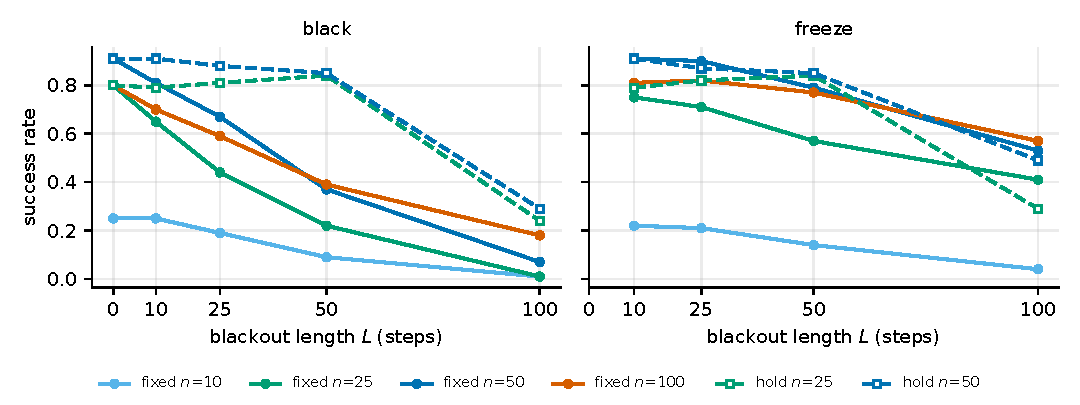
\includegraphics[width=\textwidth]{figs/fig_grid}
\caption{TC success rate against blackout length. Solid: \fixed($n$) on the LeRobot loop. Dashed: blind-aware hold on our loop. The half-width of a 95\% interval is between 0.026 and 0.096 per point.}
\label{fig:grid}
\end{figure}

With black frames and $L{=}50$, \fixed succeeds in 22, 37 and 39 of 100 episodes at $n{=}25$, 50 and 100, and at $L{=}100$ in 1, 7 and 18. With frozen frames the same cells give 57, 79 and 77 at $L{=}50$ and 41, 53 and 57 at $L{=}100$. Short blackouts are cheap for frozen frames: at $L{=}25$ and $n{=}50$ the success is 90/100, close to the 91/100 of the clean runs. Black frames are worse than frozen frames in every cell with $L\ge25$ and $n\ge25$.

\subsection{With black frames the damage tracks replans on the bad image, and one bad replan costs more at larger $n$}
\label{sec:res-mech}

The number $k$ of replans inside the window (Eq.~\ref{eq:k}) depends on $n$, $L$ and the phase of the onset. At $n{=}100$ and $L{=}50$ the phase alone decides whether a replan falls inside the window, so the 100 episodes of that cell split into 43 with $k{=}0$ and 57 with $k\ge1$. With black frames, the episodes with $k{=}0$ succeed 36 times out of 43 and those with $k\ge1$ 3 times out of 57. With frozen frames the split is 36/43 against 41/57 (Fig.~\ref{fig:mech}a). In the $k{=}0$ episodes the policy never sees a changed image, so the two faults are the same experiment there, which is why both give 36/43. The difference at $k\ge1$ is therefore a difference in what the replan ingested, not in whether a replan happened. The same pattern appears at $L{=}25$ (black 2/30, frozen 25/30 with $k\ge1$; 57/70 for both with $k{=}0$) and at $L{=}10$ (0/12 and 11/12; 70/88 for both). The onset also decides where in the task the blackout falls, so this comparison is confounded with task phase; the intervention in Sec.~\ref{sec:res-hold} addresses that, because both of its arms use the same seeds and onsets.

\begin{figure}[t]
\centering
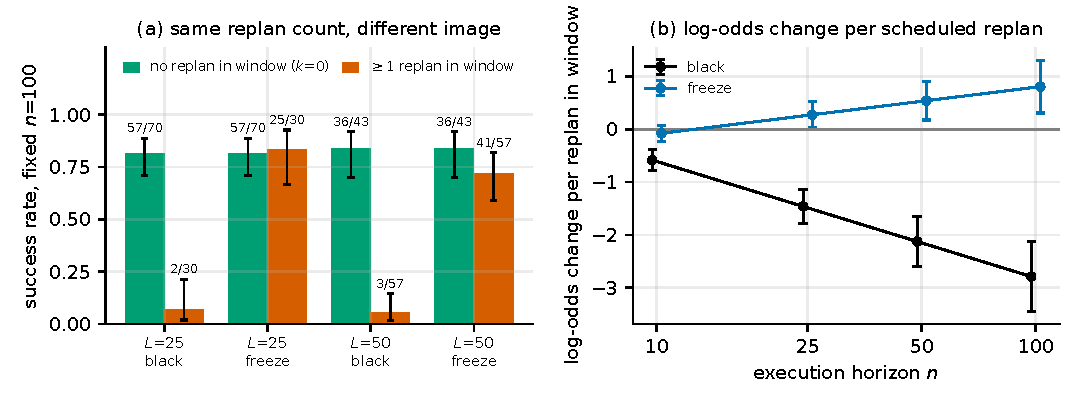
\includegraphics[width=\textwidth]{figs/fig_mech}
\caption{(a) \fixed(100) on TC at $L{=}25$ and $50$, split by whether a replan falls inside the window; error bars are 95\% Wilson intervals. (b) Change in log-odds of success per additional scheduled replan inside the window (Eq.~\ref{eq:k}), for each $n$, from a logistic regression with $k$, $\log_2 n$, their product and $L$ (1600 episodes per fault type, standard errors clustered by seed).}
\label{fig:mech}
\end{figure}

A logistic regression on the grid with $n\in\{10,25,50,100\}$ and $L\in\{10,25,50,100\}$ (1600 episodes per fault type) lets the cost of a replan depend on $n$. With $k$ from Eq.~\ref{eq:k}, the interaction of $k$ and $\log_2 n$ for black frames is $-0.66$ (cluster-robust standard error 0.097). The log-odds change per additional replan inside the window is $-0.58$ at $n{=}10$, $-1.46$ at $n{=}25$, $-2.12$ at $n{=}50$ and $-2.79$ at $n{=}100$ (odds ratios 0.56 to 0.06). Using only the cells in which $L$ is not a multiple of $n$, where the phase of the onset alone decides $k$, the log odds ratio for one more replan is $-0.99$ at $n{=}10$, $-1.43$ at $n{=}25$, $-2.43$ in both such cells at $n{=}50$ and $-3.88$ to $-4.56$ in the three at $n{=}100$ (0.5 added to each count). Adding the onset $t_0$ and $t_0^2$ to the regression changes the black slopes to $-0.62$ to $-3.05$, which does not alter this picture. For frozen frames the slopes are $-0.08$, $+0.27$, $+0.54$ and $+0.81$, and the intervals for $n\ge25$ lie above zero (Fig.~\ref{fig:mech}b); they do not change with $t_0$ and $t_0^2$. The phase-only log odds ratios for frozen frames, however, have both signs ($-0.66$ to $+0.70$ over seven cells). We therefore report the positive frozen slope only as an association in this grid, in which $k$ is tied to the phase of the onset, and not as evidence that replanning on a frozen frame helps. We use the scheduled count because the logged count is lower only in episodes that succeed inside the window, so it depends on the outcome; with the logged count the black slopes barely move ($-0.56$ to $-2.92$) and the frozen intervals for $n\ge25$ contain zero. With black frames, then, horizon and blackout length interact: $L$ and $n$ together set how many bad replans occur, roughly $L/n$, and $n$ sets how long each bad plan is executed. We read the larger slope at larger $n$ as the consequence of executing a plan made from a black image for longer. This reading is consistent with the data but we did not test it directly.

\subsection{Not replanning inside the window recovers most of the black-frame loss for $L\le50$, but with frozen frames at $L{=}100$ it is worse than leaving the policy alone}
\label{sec:res-hold}

Table~\ref{tab:hold} compares \hold and \detect with \fixed in the same loop. With black frames and $L\le50$, \hold returns success to near the clean rate. At $L{=}50$ it reaches 84/100 at $n{=}25$ (\fixed: 19) and 85/100 at $n{=}50$ (\fixed: 37), against 80 and 91 without blackout; recovery is $\rho=1.07$ [0.94, 1.22] and $0.89$ [0.78, 0.98], and at $n{=}50$ the two rules disagree on 60 seeds, 54 of them in favor of hold (P1). The pixel rule \detect reaches the same counts, 84 and 85, and in the 800 blackout episodes of its test it raised an alarm in the first step of every window and never outside it. Its cost without blackout is small: 89/100 against 91/100 for \fixed(50) in the LeRobot loop (0/2 discordant seeds). At $L{=}100$ the chunk of 100 steps runs out inside the window in most episodes (on average 0.94 forced replans at $n{=}25$ and 0.82 at $n{=}50$), and recovery is partial: 24/100 and 29/100 against 1 and 8, $\rho=0.29$ and $0.25$.

\begin{table}[t]
\centering\small
\resizebox{\textwidth}{!}{\begin{tabular}{lrrrrrrrr}
\toprule
mode & $L$ & $n$ & clean & \fixed & \hold & $\rho$ (hold) & hold/fixed & \detect \\
\midrule
black & 25 & 25 & 80/100 & 44/100 & 81/100 & 1.03 [0.89, 1.21] & 43/6 & 82/100 \\
black & 25 & 50 & 91/100 & 66/100 & 88/100 & 0.88 [0.72, 1.00] & 24/2 & 88/100 \\
black & 50 & 25 & 80/100 & 19/100 & 84/100 & 1.07 [0.94, 1.22] & 68/3 & 84/100 \\
black & 50 & 50 & 91/100 & 37/100 & 85/100 & 0.89 [0.78, 0.98] & 54/6 & 85/100 \\
black & 100 & 25 & 80/100 & 1/100 & 24/100 & 0.29 [0.19, 0.41] & 23/0 & 21/100 \\
black & 100 & 50 & 91/100 & 8/100 & 29/100 & 0.25 [0.15, 0.36] & 24/3 & 28/100 \\
\midrule
freeze & 25 & 25 & 80/100 & 70/100 & 82/100 & 1.20 [0.71, 1.54]$^*$ & 15/3 & 82/100 \\
freeze & 25 & 50 & 91/100 & 88/100 & 87/100 & n/r & 1/2 & 88/100 \\
freeze & 50 & 25 & 80/100 & 53/100 & 84/100 & 1.15 [0.86, 1.55] & 35/4 & 86/100 \\
freeze & 50 & 50 & 91/100 & 77/100 & 85/100 & 0.57 [0.17, 0.93]$^*$ & 12/4 & 85/100 \\
freeze & 100 & 25 & 80/100 & 40/100 & 29/100 & -0.28 [-0.62, -0.03] & 8/19 & 29/100 \\
freeze & 100 & 50 & 91/100 & 54/100 & 49/100 & -0.14 [-0.42, 0.08] & 7/12 & 49/100 \\
\bottomrule
\end{tabular}
}
\caption{TC, \fixed against \hold and \detect on one loop; the clean column, and so the denominator of $\rho$, comes from the LeRobot loop. Counts are successes out of 100. $\rho$ is recovery (Eq.~\ref{eq:rho}) with 95\% bootstrap interval; ``n/r'': denominator below 0.10; $^*$: more than 5\% of the bootstrap resamples had a denominator below 0.10. hold/fixed: seeds where only hold / only fixed succeeds.}
\label{tab:hold}
\end{table}

The intervention also separates the replan itself from the horizon. Among the 200 pairs of episodes with $L\in\{25,50\}$, those where \fixed(100) would replan inside the window ($k{\ge}1$, 87 pairs) and those where it would not (113), \hold($n{=}50$) with black frames wins on the first group (75/87 against 5/87 for \fixed(100)) and not on the second (98/113 against 93/113). The gain sits where a bad replan would have happened, and it is not an effect of a larger $n$. For frozen frames the corresponding gain is smaller (74/87 against 66/87).

The frozen-frame cells do not support a one-sided story. At $L{=}50$ hold still helps at $n{=}25$ (84 against 53, 35/4) but not significantly at $n{=}50$ (85 against 77, 12/4, uncorrected $p=0.077$). At $L{=}100$ it is lower than \fixed at both horizons of Table~\ref{tab:hold}: 29 against 40 at $n{=}25$ (8/19) and 49 against 54 at $n{=}50$ (7/12). Hold was also run at $n\in\{1,10\}$, where clean success is at most 25/100 and it is above the LeRobot-loop \fixed\ (1 against 0, 9 against 4), and at $n{=}100$ it is the same rule as \fixed. We repeated the $n{=}50$ cell on 100 fresh seeds (150--249): hold succeeds in 39 episodes and \fixed in 55, with 1/17 discordant seeds, that is, 17 of the 18 in favor of \fixed\ (P2, $p_{\mathrm{Holm}}=4.3\times10^{-4}$). A plausible reason, which we did not test, is that the forced replan at the end of the window then uses a frame that is up to 100 steps stale together with a joint state that has moved on, whereas \fixed replans earlier on the same frame while the state is still close to it. With black frames, replanning on the bad image is sufficient to explain most of the loss for $L\le50$, and \hold removes most of it. With frozen frames at $L{=}100$, replanning on the image is not the main cost, and not replanning is the worse choice.

\subsection{A second task repeats the black-frame intervention at a lower absolute level}
\label{sec:res-ins}

On Insertion the clean success rate is low (25/200 at $n{=}25$, 36/200 at $n{=}50$, 41/200 at $n{=}100$ with reward${=}4$), so absolute differences are small. Table~\ref{tab:ins} gives \fixed in the same loop, \hold, and \detect. With black frames and $L{=}50$, hold raises success from 9 to 24 of 200 at $n{=}25$ and from 6 to 31 at $n{=}50$, and \detect from 9 to 26 and from 6 to 32. The pre-registered family F1 tests hold at $n{=}25$, \detect at $n{=}25$ and hold at $n{=}50$ against the rerun of \fixed, and all three hold after Holm correction ($p_{\mathrm{Holm}}=0.0091$, $0.0091$ and $3.3\times10^{-5}$). The hold and \detect arms are first-study rows on the same seeds, so this shows that the two borderline $n{=}25$ cells survive a rerun of \fixed; it is not an independent replication. The recovery at $n{=}50$ is $\rho=0.83$ [0.58, 1.15]; it is not reported at $n{=}25$ because the clean-minus-fixed gap is 0.08. The post hoc metric reward${\ge}3$ shows the same picture with more power: at $n{=}50$ the counts are 33 for \fixed, 118 for \hold and 121 clean ($\rho=0.97$ [0.88, 1.06]). At $L{=}100$ recovery is partial, as on TC (reward${\ge}3$, $\rho=0.47$ and $0.43$). The natural experiment of Sec.~\ref{sec:res-mech} also repeats: with \fixed(100), $L{=}50$ and black frames, episodes without a replan in the window succeed in 23 of 96 and those with one in 0 of 104 (frozen: 23/96 and 15/104).

\begin{table}[t]
\centering\small
\resizebox{\textwidth}{!}{\begin{tabular}{lrrrrrrrr}
\toprule
mode & $L$ & $n$ & clean & \fixed & \hold & \detect & $\rho$ (hold) & hold/fixed \\
\midrule
\multicolumn{9}{l}{\emph{reward${=}4$ (primary)}} \\
black & 50 & 25 & 25/200 & 9/200 & 24/200 & 26/200 & n/r & 22/7 \\
black & 50 & 50 & 36/200 & 6/200 & 31/200 & 32/200 & 0.83 [0.58, 1.15] & 29/4 \\
black & 100 & 25 & 25/200 & 1/200 & 6/200 & 6/200 & 0.21 [0.04, 0.40]$^*$ & 5/0 \\
black & 100 & 50 & 36/200 & 0/200 & 6/200 & 6/200 & 0.17 [0.05, 0.33] & 6/0 \\
freeze & 50 & 25 & 25/200 & 18/200 & 24/200 & 22/200 & n/r & 15/9 \\
freeze & 50 & 50 & 36/200 & 25/200 & 33/200 & 34/200 & n/r & 18/10 \\
freeze & 100 & 25 & 25/200 & 10/200 & 8/200 & 7/200 & n/r & 4/6 \\
freeze & 100 & 50 & 36/200 & 15/200 & 10/200 & 11/200 & -0.24 [-0.50, 0.10]$^*$ & 4/9 \\
\midrule
\multicolumn{9}{l}{\emph{reward${\ge}3$ (post hoc)}} \\
black & 50 & 25 & 98/200 & 25/200 & 92/200 & 93/200 & 0.92 [0.79, 1.06] & 71/4 \\
black & 50 & 50 & 121/200 & 33/200 & 118/200 & 116/200 & 0.97 [0.88, 1.06] & 92/7 \\
black & 100 & 25 & 98/200 & 4/200 & 48/200 & 48/200 & 0.47 [0.36, 0.58] & 44/0 \\
black & 100 & 50 & 121/200 & 7/200 & 56/200 & 56/200 & 0.43 [0.33, 0.54] & 50/1 \\
freeze & 50 & 25 & 98/200 & 74/200 & 89/200 & 89/200 & 0.63 [0.27, 0.96]$^*$ & 23/8 \\
freeze & 50 & 50 & 121/200 & 110/200 & 117/200 & 118/200 & n/r & 22/15 \\
freeze & 100 & 25 & 98/200 & 43/200 & 37/200 & 38/200 & -0.11 [-0.35, 0.07] & 10/16 \\
freeze & 100 & 50 & 121/200 & 80/200 & 71/200 & 72/200 & -0.22 [-0.56, 0.02] & 8/17 \\
\bottomrule
\end{tabular}
}
\caption{Insertion (200 seeds). Counts are successes; \fixed is the same-loop rerun. Top: reward${=}4$, the primary metric. Bottom: reward${\ge}3$, a post hoc secondary metric. Notation as in Table~\ref{tab:hold}.}
\label{tab:ins}
\end{table}

The frozen-frame half of the TC result also appears on Insertion, with weaker evidence. At $L{=}50$ neither rule changes the primary metric by more than 0.05 (the largest absolute difference to \fixed is 0.045). At $L{=}100$ the point estimates of hold are at or below those of \fixed in all four cells and both metrics (for example 10 against 15 of 200 at $n{=}50$ with reward${=}4$, and 71 against 80 with reward${\ge}3$), none of the differences is significant, and we do not rest a claim on them.

\subsection{A detector trained on clean frames covers three corruptions it was designed against and one it was not, and fails on two others}
\label{sec:res-ood}

Table~\ref{tab:syn} and Fig.~\ref{fig:corr} show the synthetic and unseen corruptions at $n{=}50$ and $L{=}50$. The hold rule never receives a corrupted frame at this setting, so its outcome does not depend on which corruption is applied. At $n{=}50$, $L{=}50$ its 75/90 successes are identical seed by seed for noise, occlusion, delay and flicker (0 of 90 episodes differ), and at $n{=}25$ the rows differ by at most 4 of 90 episodes because of rendering noise. We therefore count the four hold rows as one experiment, not four replications. What the corruptions test is how bad the fault is for \fixed\ (retention 0.46 to 0.75 for the four synthetic corruptions) and whether a detector can see it.

\begin{table}[t]
\centering\small
\resizebox{\textwidth}{!}{\begin{tabular}{llrrrrrrr}
\toprule
corruption & status & clean & \fixed & \hold & \ood & $\rho$ (hold) & $\rho$ (\ood) & flagged \\
\midrule
noise $\sigma{=}0.6$ & probe set & 81/90 & 37/90 & 75/90 & 75/90 & 0.86 [0.73, 0.98] & 0.86 [0.73, 0.98] & 1.00 \\
occlusion 0.5 & probe set & 81/90 & 40/90 & 75/90 & 75/90 & 0.85 [0.71, 0.98] & 0.85 [0.71, 0.98] & 1.00 \\
flicker $p{=}0.6$ & probe set & 81/90 & 61/90 & 75/90 & 77/90 & 0.70 [0.36, 0.95] & 0.80 [0.57, 0.96] & 0.46 \\
delay $d{=}50$ & not in probe set & 81/90 & 53/90 & 75/90 & 52/90 & 0.79 [0.55, 0.96] & -0.04 [-0.14, 0.00] & 0.04 \\
blur $\sigma{=}40$ & unseen, pre-reg. & 79/90 & 35/90 & 75/90 & 74/90 & 0.91 [0.80, 1.00] & 0.89 [0.77, 1.00] & 1.00 \\
dim $g{=}0.1$ & unseen, pre-reg. & 79/90 & 48/90 & 75/90 & 53/90 & 0.87 [0.70, 1.00] & 0.16 [0.00, 0.33] & 0.16 \\
\bottomrule
\end{tabular}
}
\caption{Synthetic and unseen corruptions, TC, $n{=}50$, $L{=}50$, 90 seeds. The \hold column repeats one experiment in the first four rows (identical outcomes); blur and dim have their own hold runs, which also give 75/90. ``Flagged'': share of in-window steps flagged by the OOD detector. ``Clean'' for blur and dim is the same-loop clean rate; for the others it is the clean rate of the LeRobot loop. Notation as in Table~\ref{tab:hold}.}
\label{tab:syn}
\end{table}

\begin{figure}[t]
\centering
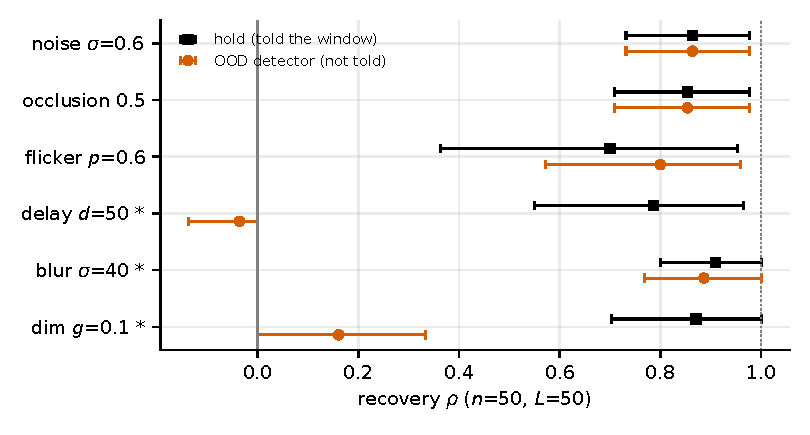
\includegraphics[width=0.75\textwidth]{figs/fig_corr}
\caption{Recovery $\rho$ of hold (told the window) and of the OOD detector (not told) at $n{=}50$, $L{=}50$, with 95\% bootstrap intervals. Starred rows are corruptions that were not among the frames used to design the detector.}
\label{fig:corr}
\end{figure}

The detector flags every in-window step for noise, occlusion and blur, and recovers as much as hold does: 75, 75 and 74 successes of 90, against 37, 40 and 35 for \fixed\ ($\rho=0.86$, $0.85$ and $0.89$). For flicker it flags 46\% of the in-window steps and recovers $\rho=0.80$ [0.57, 0.96]; at $L{=}100$ it does better than hold (79 against 65 of 90, 16/2 discordant, exploratory $p=0.0013$), perhaps because it holds back only on bad frames and still replans on good ones; we did not test this. It fails on two corruptions. Delayed frames are real frames from the past, the flagged share (0.038) is close to the false-alarm rate of 0.028, and the recovery is $-0.04$ [$-0.14$, 0.00], although hold recovers $0.79$ [0.55, 0.96]. On dimmed images ($g{=}0.1$) it flags 16\% of in-window steps and recovers $\rho=0.16$ [0.00, 0.33], against $0.87$ for hold, and only 34\% of the dim episodes contain any alarm. The pre-registered criterion for ``not general'' was a flagged share below 0.30 or a recovery below 0.30 for either unseen corruption with enough damage; dim triggers both (Appendix~\ref{app:extra} lists all pre-registered predictions). The pre-registered contrast on blur holds ($p_{\mathrm{Holm}}$ in Table~\ref{tab:primary}) and the one on dim does not (6/1 discordant seeds, $p_{\mathrm{Holm}}=0.125$). Of the three corruptions that were not among the design frames (delay, blur, dim), the detector handles one. We therefore do not call it general, and we present it as a detector for corruptions that make frames statistically unlike clean ones.

The false-alarm rate is a second limit. We set the threshold for 1\% of clean frames; on the unseen-corruption runs the rate outside the window is 3.3\% (blur) and 2.7\% (dim), and across the synthetic experiments it lies between 1.6\% and 4.3\% by cell. Between 16\% and 24\% of the clean episodes contain at least one false alarm. This costs little: with no blackout the success of \ood and \fixed differs by $+0.022$, $0.000$ and $0.000$ at $n{=}25$, 50 and 100 (Appendix~\ref{app:extra}). The pixel rule \detect, by contrast, never fires on noise, occlusion or delay (0 flagged steps in 540 episodes), as designed; it was not run on flicker. The detector's design was not a single attempt: its first version, a Mahalanobis distance inside the principal subspace, failed on the probe corruptions (in-window score medians were not above the clean median, and black frames were never detected), and the reconstruction-error score was chosen from seven variants compared on probe frames from the pilot seeds (Appendix~\ref{app:protocol}). Detection rates and the AUC against a ``harmful to the policy'' label were computed on the development seeds 120--149 only.

\subsection{Median TE is close to hold on short black windows and beats hold on long frozen ones; a CARE-style trigger does not help}
\label{sec:res-base}

\begin{table}[t]
\centering\small
\resizebox{\textwidth}{!}{\begin{tabular}{lrrrrrrr}
\toprule
rule & clean & black 25 & black 50 & black 100 & freeze 50 & freeze 100 & calls/ep \\
\midrule
\fixed(50) & 91 & 66 & 37 & 8 & 77 & 54 & 7.5 \\
\fixed(100) & 80 & 59 & 39 & 17 & 77 & 56 & 3.7 \\
\hold(50) & 91 & 88 & 85 & 29 & 85 & 49 & 6.5 \\
Mean TE, $h{=}1$ & 83 & 53 & 35 & 7 & 82 & 58 & 365.3 \\
Median TE, $h{=}1$ & 83 & 85 & 54 & 5 & 81 & 74 & 365.6 \\
Median TE, $h{=}10$ & 84 & 86 & 53 & 8 & 86 & 63 & 36.9 \\
CARE-style, $\tau{=}0.3$ & 84 & 54 & 23 & 9 & 67 & 46 & 14.5 \\
\bottomrule
\end{tabular}
}
\caption{TC, literature baselines against \fixed and \hold on the same loop, 100 seeds, except that the clean column of \fixed and Mean TE comes from the LeRobot loop. Counts are successes. Column headers give fault and $L$. ``calls/ep'': mean number of policy calls per episode in the freeze, $L{=}100$ cell. The clean column of \hold is that of \fixed(50).}
\label{tab:base}
\end{table}

Table~\ref{tab:base} compares the literature baselines with \fixed and \hold. Median TE with $h{=}1$ is close to hold for short black windows (85 against 88 at $L{=}25$, 10/13 discordant, no difference) and far above Mean TE (53). It falls to the level of \fixed at $L{=}100$ (5 against 8). At $L{=}50$ it is above \fixed(50) (54 against 37, 35/18, exploratory $p=0.027$) but well below hold (5/36). The case in which it does best is the one in which hold does worst, frozen frames with $L{=}100$: 74 of 100, against 54 for \fixed(50) (29/9, exploratory $p=0.0017$) and 49 for hold (33/8). On 100 new seeds the comparison with hold repeats (Median TE 60, hold 39, 31/10, $p_{\mathrm{Holm}}$ in Table~\ref{tab:primary}) but the comparison with \fixed(50) does not (60 against 55, 27/22, $p=0.57$), which was a pre-registered prediction that fails. The advantage over hold, not over leaving the policy alone, is what is confirmed. Median TE also needs per-step queries: 374 policy calls per episode at $h{=}1$ and 37 at $h{=}10$ in the confirmatory cell, against 6.5 for hold and 7.7 for \fixed(50), and with $h{=}10$ the success is 62 against 60 (15/13, no difference).

The CARE-style trigger brings no gain. With the main threshold $\tau{=}0.3$ it scores below \fixed(50) in four of five cells, for example 23 against 37 at black $L{=}50$ ($\rho=-0.26$ [$-0.49$, $-0.08$]) and 67 against 77 at freeze $L{=}50$, and equal in the cell where nothing works (black $L{=}100$: 9 against 8). Part of the gap is a clean cost: with this $\tau$, CARE succeeds in 84 of 100 clean episodes against 91 for \fixed(50). Measured against its own clean rate the retention is still lower (black $L{=}50$: 0.27 against 0.41). A looser $\tau$ narrows the gap (32 at $\tau{=}0.5$), and none of the three thresholds beats \fixed(50) (Appendix~\ref{app:extra}). This statement is about our adaptation. CARE was designed for brief perturbations, our blackouts last 25 to 100 steps, and $\tau$ is our own calibration, so we do not conclude that CARE is harmful.

%==============================================================================
\section{Discussion and Limitations}
\label{sec:discussion}

Hold is a mechanism test. Where it works (black frames, $L\le50$ on TC and $L{=}50$ on Insertion) it shows that the replans inside the window account for most of the loss: recovery at $L{=}25$ and 50 is 0.88 to 1.07 on TC and 0.83 on Insertion at $n{=}50$. It does not show that hold is a good controller, since it needs to be told the window, and where it fails (frozen frames, $L{=}100$) the information that the image is stale was not enough. The within-cell comparison, the regression and the intervention look at the same cause from three sides and are not three independent confirmations: the first two use the same episodes, and all three rest on the same seeds. For black frames our conclusion is that replanning on the bad image is sufficient to explain most of the loss at $L\le50$. We do not claim it is the only cause at $L{=}100$, where hold recovers only 0.25 to 0.29 of the loss on TC.

Suh et al.~\cite{suh2026blackout} report that on VLAs both faults give low success with different failure modes, and in their pooled table frozen frames are the worse fault (scene camera, with proprioception: $\pi_{0.5}$ 5.8\% frozen against 28.9\% black, GR00T 9.3\% against 51.6\%). In our ACT results black is the more damaging fault in every cell with $L\ge25$ and $n\ge25$. We can offer hypotheses that we did not test: a black image is far from anything ACT's visual encoder saw in training, while a frozen frame is a plausible scene, and a frozen frame taken at the start of an episode (as in their episode-start faults) conveys that nothing has happened, whereas ours is taken at the onset of the window. The setups differ in model, task, fault duration and what the policy receives, so we do not claim a disagreement.

Median TE and CARE were designed for sparse or momentary corruption. Our blackouts corrupt 25 to 100 consecutive steps. Median TE beat hold in the one regime where hold hurts, but on fresh seeds it did not beat \fixed(50), and $h{=}10$ matched $h{=}1$ there (62 against 60) with 37 policy calls instead of 374. We report CARE's lower scores as a property of our adaptation, with a $\tau$ we calibrated ourselves. A trigger based on proprioceptive tracking error, which we tried before this work, did not help either (Appendix~\ref{app:extra}).

We also tried to train a Diffusion Policy on the same demonstrations (LeRobot 0.4.4; a search of the \texttt{lerobot} organization on the Hugging Face Hub on 2026-11-06 returned two Diffusion Policy checkpoints, both for PushT, and two ALOHA checkpoints, both ACT) to repeat the grid on a different architecture. It did not produce a policy good enough to test. At the pre-declared gate of 20 episodes without blackout, the 20k-step run (v1) succeeded in 0/20 episodes, a 40k-step run with EMA and the original simulation settings (horizon 16, v2) in 0/20 (2 episodes lifted the cube), and a 20k-step run on scripted demonstrations (v3) in 0/20 (Wilson upper bound 0.16 each). We extended v2 to 100k steps, the length of its learning-rate schedule, and it succeeded in 2/20 episodes (0.10, Wilson 95\% CI 0.03 to 0.30), below the 0.30 we had set before this run as the minimum for running the grid. We therefore stopped and did not run the blackout grid on it. This says only that our training did not yield a usable policy within budget, not that Diffusion Policy cannot do this task. No conclusion above uses it, and our results are restricted to ACT.

\paragraph{Limitations.} (1) Everything is simulated; real cameras fail in other ways and real latency matters. (2) We use pretrained ACT checkpoints for two tasks and no other policy family, so the interaction of $n$ and $L$ is shown for one architecture. (3) Corruption strengths were chosen by us from a 30-episode pilot whose retention estimates are uncertain by about $\pm0.15$--$0.2$; the four synthetic strengths give a retention of 0.46 to 0.75 for \fixed(50), against 0.41 for black frames in the same cell. (4) Insertion's clean success is 12.5\% to 20.5\%, its reward-4 criterion is a contact event about 2 cm inside a 12 cm socket that does not require the peg to be aligned; we rely on the secondary metric for power, and it is post hoc. (5) Seeds are shared across cells, so neighboring cells are not independent replications, and we never treat them as such. (6) The OOD detector was designed while looking at noise, occlusion, black frames and flicker; its false-alarm rate is above its target. Severity and detectability are confounded, because the selected strengths are severe and full detection is partly by design; we did not sweep strengths, and the harmful faults that the detector cannot see are delay and frozen frames. (7) Episode-level outcomes are not reproducible across execution loops, so only marginal success rates are claimed. (8) The six-row list in Table~\ref{tab:primary} was assembled after all runs; P1 and P2 are not pre-registered as primary contrasts, and the pre-registration lists the comparison in P2 as exploratory. The pre-registered families were written after the first study, and the public repository cannot show when. (9) Several literature results are single preprints that may not have been peer reviewed. (10) The explanations offered for hold's failure with frozen frames, for the growth of the per-replan cost with $n$, and for the black-frozen ordering are hypotheses, not tested results.

%==============================================================================
\section{Conclusion}
\label{sec:conclusion}

Whether a chunked policy should replan during a camera fault depends on what the fault shows it. For black frames in simulated ACT policies, replanning inside the window explains most of the loss for windows up to 50 steps, not replanning returns success to near the clean rate on two tasks, and on Transfer Cube one such replan costs more at larger execution horizons. For frozen frames the same rule is not safe at $L{=}100$. A detector trained on clean frames can supply the signal for several corruptions but not for delayed, dimmed or frozen frames, where dimming triggered the pre-registered criterion for calling it not general, and its false-alarm rate is above its target. For practitioners, the cheapest mitigation for black frames is not to replan while the camera is known or detected to be bad; for frozen frames at $L{=}100$ we found no rule that reliably beats leaving the policy alone: Median TE beat hold there, but not \fixed(50) on fresh seeds. What a real-robot test would need to show is that the same ordering holds with real camera faults and a detector that does not depend on the faults we designed it against.

\paragraph{Use of generative AI.} The experiment code, the analysis and the text of this paper were largely written by Claude (Anthropic), an AI assistant, under the author's direction and review. The author takes responsibility for the content.

%==============================================================================
\bibliographystyle{plainnat}
\bibliography{refs}

\appendix
\section{Appendix}

\subsection{Protocol details}\label{app:protocol}
\paragraph{Corruption strengths.} Table~\ref{tab:pilot} lists every pilot result. \fixed(50), $L{=}50$, seeds 120--149; clean reference 24/30 on the same seeds. Selected strengths are noise $\sigma{=}0.6$, occlusion 0.5 of the frame area centered (a tie with 0.75 centered, the weaker was taken), delay $d{=}50$ and flicker $p{=}0.6$, then blur $\sigma{=}40$ and dim $g{=}0.1$. For dim, $g{=}0.1$ was the only strength inside $[0.15,0.85]$; the pre-registered fourth strengths (blur $\sigma{=}80$, dim $g{=}0.03$) were not needed. Our notes record the rule as fixed before the pilot for the first four corruptions, with one clause added after the pilot results were seen (flicker $p{=}1$ excluded); for blur and dim it is in the pre-registration in full. As above, the public repository cannot date either.
\begin{table}[h]
\centering\small
\begin{tabular}{lrrl}
\toprule
corruption and strength & \fixed(50) success & $R$ &  \\
\midrule
noise $\sigma{=}0.1$ & 21/30 & 0.87 &  \\
noise $\sigma{=}0.3$ & 18/30 & 0.75 &  \\
noise $\sigma{=}0.6$ & 12/30 & 0.50 & selected \\
occlusion 0.25 center & 18/30 & 0.75 &  \\
occlusion 0.5 center & 15/30 & 0.62 & selected \\
occlusion 0.75 center & 15/30 & 0.62 &  \\
occlusion 0.25 random & 20/30 & 0.83 &  \\
occlusion 0.5 random & 17/30 & 0.71 &  \\
occlusion 0.75 random & 16/30 & 0.67 &  \\
delay $d{=}5$ & 23/30 & 0.96 &  \\
delay $d{=}25$ & 22/30 & 0.92 &  \\
delay $d{=}50$ & 15/30 & 0.62 & selected \\
flicker $p{=}0.3$ & 21/30 & 0.87 &  \\
flicker $p{=}0.6$ & 19/30 & 0.79 & selected \\
flicker $p{=}1.0$ & 18/30 & 0.75 &  \\
blur $\sigma{=}5$ (unseen) & 19/30 & 0.79 &  \\
blur $\sigma{=}15$ (unseen) & 17/30 & 0.71 &  \\
blur $\sigma{=}40$ (unseen) & 11/30 & 0.46 & selected \\
dim $g{=}0.5$ (unseen) & 23/30 & 0.96 &  \\
dim $g{=}0.25$ (unseen) & 24/30 & 1.00 &  \\
dim $g{=}0.1$ (unseen) & 19/30 & 0.79 & selected \\
\bottomrule
\end{tabular}

\caption{Pilot for corruption strength. $R$: success of \fixed(50) divided by the clean success on the same seeds (30 episodes each).}
\label{tab:pilot}
\end{table}

\paragraph{OOD detector.} The principal subspace has 16 components on 6144-dimensional pooled features and was fit on 3,434 frames of clean episodes with seeds 100--109 (explained variance 0.81). The threshold $\theta=28.29$ is the 99th percentile of the score on 3,335 frames of clean episodes with seeds 110--119. The detector was frozen by hash before the P2b runs. The first version used the Mahalanobis distance inside the subspace and failed: the in-window score medians of its probe corruptions (2.6--3.9) were not above the median of clean scores (3.8), and the detection rate for black frames was zero. It was replaced after comparing seven variants (squared prediction error, $T^2$, k-nearest-neighbor distance and others) on static starting frames of six probe seeds (120--125) corrupted by noise ($\sigma=0.6,0.3$), occlusion (0.5, 0.25), black and flicker. This replacement used the pilot seeds and not the evaluation seeds, and no parameter was tuned on the evaluation seeds. On the development seeds we also measured detection against a harmfulness label (the detector flags 1.000 of harmful black steps and 0.034 of harmful frozen steps): a frame is harmful if the chunk predicted from it differs from the chunk predicted from the true frame by more than the 99th percentile of the difference caused by $\pm1$ gray-level jitter, which is 0.0317 rad. On the development seeds the AUC of the score against this label is 0.991 for flicker and 0.537 for frozen frames. The flagged shares per corruption on the evaluation seeds are in Table~\ref{tab:detector}.

\paragraph{CARE thresholds.} $\tau$ was calibrated in a closed loop on clean seeds 100--119 to give a mean executed length near 30 steps (0.6 of $H_{\max}$; main, $\tau{=}0.3$), 20 steps ($\tau{=}0.18$) or 40 steps ($\tau{=}0.5$); the closed-loop runs gave 31.5, 20.9 and 38.5 steps. A first calibration on open-loop curves gave executed lengths shorter than targeted and was replaced by the closed-loop one. $\tau{=}1.0$ and $1.5$ from the original paper do not apply to ACT, whose discrepancy ratios are of order $10^{-2}$.

\paragraph{Execution and software.} Python 3.10, PyTorch 2.10, LeRobot 0.4.4, gym-aloha 0.1.5, MuJoCo 3.8.1, EGL rendering, one NVIDIA RTX 5070 Ti. The grid for TC was run with LeRobot's action queue; later experiments use our own loop (\texttt{code/run\_p2p3.py}). Replans within a window are counted as queue-empty events.

\subsection{Insertion details}\label{app:ins}
Table~\ref{tab:insfixed} compares the \fixed rows of the first Insertion run (LeRobot loop) with the same-loop rerun. The marginal success rates differ by at most 0.04 in the 12 cells, and the episode-level outcome flips in up to 22 of 200 episodes. Our clean runs with the same-loop code give 25, 36 and 41 successes of 200 at $n{=}25$, 50 and 100 (the first run: 32, 31 and 41). In the 200 clean episodes at $n{=}100$ the maximum reward is 0 in 33, 1 in 40, 2 in 14, 3 in 72 and 4 in 41 episodes. The model card (20.6\%) is close to our 41/200 (20.5\%) and the \path{eval_info.json} (83.0\%, 415 of 500 reaching reward 4) is not; we cannot say why.
\begin{table}[h]
\centering\small
\begin{tabular}{lrrrrr}
\toprule
mode & $L$ & $n$ & old \fixed\ (float32) & new \fixed\ (same loop) & flips \\
\midrule
black & 50 & 25 & 9/200 & 9/200 & 6 \\
black & 50 & 50 & 9/200 & 6/200 & 3 \\
black & 50 & 100 & 22/200 & 23/200 & 3 \\
black & 100 & 25 & 0/200 & 1/200 & 1 \\
black & 100 & 50 & 0/200 & 0/200 & 0 \\
black & 100 & 100 & 1/200 & 1/200 & 0 \\
freeze & 50 & 25 & 22/200 & 18/200 & 16 \\
freeze & 50 & 50 & 33/200 & 25/200 & 22 \\
freeze & 50 & 100 & 38/200 & 38/200 & 4 \\
freeze & 100 & 25 & 8/200 & 10/200 & 6 \\
freeze & 100 & 50 & 16/200 & 15/200 & 1 \\
freeze & 100 & 100 & 20/200 & 19/200 & 1 \\
\bottomrule
\end{tabular}

\caption{Insertion, reward${=}4$: old \fixed\ (LeRobot loop, float32) and the same-loop rerun (float64); ``flips'': seeds whose outcome differs.}
\label{tab:insfixed}
\end{table}

\subsection{Reproducibility of episodes}\label{app:noise}
The pipeline is not bit-deterministic: replaying the same 150 actions gives identical joint positions but rendered pixels that differ by at most one gray level, and the closed loop amplifies this. Same-code reruns of 900 pilot episodes change the outcome of 8 (0.9\%); in cells with mean success between 0.1 and 0.9 it is 8 of 650 (1.2\%). Between the two loops, with float64 actions in the new loop, the outcomes flip in 5/100 (black, $n{=}25$), 2/100 (black, $n{=}50$), 14/100 (freeze, $n{=}25$) and 2/100 (freeze, $n{=}50$) episodes at $L{=}50$, with success counts 19 against 22, 37 against 37, 53 against 57 and 77 against 79. Rerunning the LeRobot loop itself for freeze $n{=}25$ gives 2/100 flips. Table~\ref{tab:dtype} shows the ablation. Casting the new loop's actions to float32 reduces flips against the LeRobot loop from 19 to 5 in 200 episodes, below the pre-registered threshold of 8, so the numerical type is the main cause; it is not necessarily the only one, since the loops also differ in how they index the chunk. The same-loop clean references for \fixed on TC differ from the LeRobot-loop rates by at most 0.033 (70/90 against 73/90 at $n{=}25$, 79/90 against 81/90 at $n{=}50$, 70/90 against 70/90 at $n{=}100$).
\begin{table}[h]
\centering\small
\begin{tabular}{lrrrrrr}
\toprule
mode & run\_grid (f32) & new loop f64 & new loop f32 & f64 vs grid & f32 vs grid & f32 vs f64 \\
\midrule
black & 22/100 & 19/100 & 23/100 & 5 & 3 & 8 \\
freeze & 57/100 & 53/100 & 55/100 & 14 & 2 & 12 \\
\bottomrule
\end{tabular}

\caption{dtype ablation, TC, $n{=}25$, $L{=}50$, seeds 0--99. Flips are counted against the LeRobot loop (``run\_grid'') except the last column.}
\label{tab:dtype}
\end{table}

\subsection{Additional results}\label{app:extra}
\paragraph{Pre-registered families as registered.} Table~\ref{tab:fam} gives the three pre-registered families with the Holm correction inside each, as written in the pre-registration. Of the pre-registered predictions, those that failed are: for dim, a flagged share of at least 0.90 (observed 0.159) and a recovery of at least 0.60 (0.16); and P-TE3, a Median TE advantage over \fixed(50) at freeze $L{=}100$ after Holm (observed $+0.05$, $p_{\mathrm{Holm}}=0.654$). All others held: dtype (5/200 flips), clean references, F1 (three contrasts), Insertion marginals and the freeze $L{=}50$ no-effect prediction, blur (flagged 1.000, $\rho=0.89$, false alarms 0.0328), false alarms below 0.05 for dim (0.0270), clean cost, P-TE1 and P-TE2.
\begin{table}[h]
\centering\small
\begin{tabular}{llrrr}
\toprule
family & contrast & x/y & $p$ & $p_{\mathrm{Holm}}$ (within family) \\
\midrule
F1 & oracle $n{=}25$ vs fixed (Ins.\ black, $L{=}50$) & 22/7 & 0.008 & 0.009 \\
F1 & detect $n{=}25$ vs fixed & 25/8 & 0.005 & 0.009 \\
F1 & oracle $n{=}50$ vs fixed & 29/4 & 1.1e-5 & 3.3e-5 \\
F2 & OOD vs fixed, blur & 44/5 & 7.6e-9 & 1.5e-8 \\
F2 & OOD vs fixed, dim & 6/1 & 0.125 & 0.125 \\
F3 & TE $h{=}1$ vs hold, freeze $L{=}100$ & 31/10 & 0.001 & 0.004 \\
F3 & TE $h{=}1$ vs hold, black $L{=}25$ & 10/16 & 0.33 & 0.65 \\
F3 & TE $h{=}1$ vs fixed(50), freeze $L{=}100$ & 27/22 & 0.57 & 0.65 \\
\bottomrule
\end{tabular}

\caption{Pre-registered families F1--F3, in the wording of the pre-registration, where ``oracle'' is hold and ``TE'' is Median TE; $p_{\mathrm{Holm}}$ is within the family.}
\label{tab:fam}
\end{table}

\paragraph{Detector metrics and clean cost.} Table~\ref{tab:detector} shows detector metrics per corruption at $n{=}50$, $L{=}50$ and Table~\ref{tab:cleancost} the success of the OOD rule without any blackout.
\begin{table}[h]
\centering\small
\resizebox{\textwidth}{!}{\begin{tabular}{lrrrr}
\toprule
corruption & episodes detected & steps flagged in window & false-alarm rate (steps) & episodes with $\ge$1 false alarm \\
\midrule
noise & 1.00 & 1.000 & 0.0292 & 0.20 \\
occlusion & 1.00 & 1.000 & 0.0303 & 0.20 \\
flicker & 0.97 & 0.459 & 0.0334 & 0.17 \\
delay & 0.10 & 0.038 & 0.0281 & 0.21 \\
blur (unseen) & 1.00 & 1.000 & 0.0328 & 0.19 \\
dim (unseen) & 0.34 & 0.159 & 0.0270 & 0.17 \\
\bottomrule
\end{tabular}
}
\caption{OOD detector at $n{=}50$, $L{=}50$ (90 seeds).}
\label{tab:detector}
\end{table}
\begin{table}[h]
\centering\small
\begin{tabular}{lrrrrrr}
\toprule
$n$ & \fixed & \ood & $\Delta$ & ood/fixed & $p$ & false-alarm rate \\
\midrule
25 & 70/90 & 72/90 & +0.022 & 3/1 & 0.625 & 0.0380 \\
50 & 79/90 & 79/90 & +0.000 & 0/0 & 1.00 & 0.0314 \\
100 & 70/90 & 70/90 & +0.000 & 0/0 & 1.00 & 0.0277 \\
\bottomrule
\end{tabular}

\caption{Clean cost of the OOD rule, $L{=}0$, 90 seeds, TC. $\Delta$: success of \ood minus \fixed. False-alarm rate is the share of steps flagged.}
\label{tab:cleancost}
\end{table}

\paragraph{Median TE confirmation and CARE thresholds.} Table~\ref{tab:te} lists the confirmatory runs (seeds 150--249); Table~\ref{tab:care} the CARE thresholds at $L{=}50$.
\begin{table}[h]
\centering\small
\begin{tabular}{llrrrr}
\toprule
cell & rule & success & calls/ep & TE/other & $p$ (uncorrected) \\
\midrule
freeze $L{=}100$ & Median TE $h{=}1$ & 60/100 & 374.4 &  &  \\
freeze $L{=}100$ & Median TE $h{=}10$ & 62/100 & 37.3 & 13/15 & 0.85 \\
freeze $L{=}100$ & \fixed(50) & 55/100 & 7.7 & 27/22 & 0.57 \\
freeze $L{=}100$ & \fixed(100) & 53/100 & 3.7 & 30/23 & 0.41 \\
freeze $L{=}100$ & \hold(50) & 39/100 & 6.5 & 31/10 & 0.001 \\
\midrule
black $L{=}25$ & Median TE $h{=}1$ & 80/100 & 341.4 &  &  \\
black $L{=}25$ & Median TE $h{=}10$ & 80/100 & 33.9 & 7/7 & 1.00 \\
black $L{=}25$ & \fixed(50) & 63/100 & 7.1 & 28/11 & 0.009 \\
black $L{=}25$ & \fixed(100) & 58/100 & 3.6 & 32/10 & 9.4e-4 \\
black $L{=}25$ & \hold(50) & 86/100 & 6.5 & 10/16 & 0.33 \\
\bottomrule
\end{tabular}

\caption{Median TE confirmation on 100 new seeds. ``TE/other'': seeds where only Median TE ($h{=}1$) / only the other rule succeeds. $p$ is uncorrected.}
\label{tab:te}
\end{table}
\begin{table}[h]
\centering\small
\begin{tabular}{lrrrrr}
\toprule
$\tau$ & clean & black $L{=}50$ & freeze $L{=}50$ & $R$ black & $R$ freeze \\
\midrule
0.18 & 74 & 22 & 49 & 0.30 & 0.66 \\
0.3 & 84 & 23 & 67 & 0.27 & 0.80 \\
0.5 & 89 & 32 & 70 & 0.36 & 0.79 \\
\fixed(50) & 91 & 37 & 77 & 0.41 & 0.85 \\
\bottomrule
\end{tabular}

\caption{CARE-style trigger at three thresholds, TC, 100 seeds, successes at $L{=}50$ and retention against each rule's own clean rate.}
\label{tab:care}
\end{table}

\paragraph{A proprioceptive trigger (negative result).} Before the work above we tried replanning early when the commanded and measured joint positions disagree. The signal was $e_t=\lVert a_{t-1}-q_t\rVert_2$ over the 12 arm joints (the gripper dimensions explained 98\% of the squared error and were dropped, a choice made after seeing calibration data and before the evaluation), the threshold $\tau=0.159$ was the 99th percentile on clean seeds 100--119 at $n{=}100$, and the rule replans when $e_t>\tau$ after at least $m\in\{1,10\}$ steps of the current chunk. It does not know the window. It was not distinguishable from \fixed(50) in any cell after correction (Table~\ref{tab:proprio}; its comparison rows come from the LeRobot-loop \fixed, so this is a cross-loop comparison), and the signal does not distinguish task phases (mean 0.034 in reward stage 0 and 0.038 in stage 2). The one nominal difference, $m{=}10$ against \fixed(50) at black $L{=}100$ ($p=0.041$ uncorrected), is not a result we rely on.
\begin{table}[h]
\centering\small
\resizebox{\textwidth}{!}{\begin{tabular}{lrrrrrrrrr}
\toprule
mode & $L$ & \fixed(50) & \fixed(100) & proprio $m{=}1$ & vs 50 & $p$ & proprio $m{=}10$ & vs 50 & $p$ \\
\midrule
black & 25 & 67 & 59 & 63/100 & 14/18 & 0.60 & 63/100 & 14/18 & 0.60 \\
black & 50 & 37 & 39 & 42/100 & 29/24 & 0.58 & 42/100 & 29/24 & 0.58 \\
black & 100 & 7 & 18 & 15/100 & 13/5 & 0.096 & 17/100 & 15/5 & 0.041 \\
freeze & 25 & 90 & 82 & 87/100 & 4/7 & 0.55 & 85/100 & 4/9 & 0.27 \\
freeze & 50 & 79 & 77 & 81/100 & 12/10 & 0.83 & 80/100 & 11/10 & 1.00 \\
freeze & 100 & 53 & 57 & 57/100 & 13/9 & 0.52 & 56/100 & 12/9 & 0.66 \\
\bottomrule
\end{tabular}
}
\caption{Proprioceptive trigger, TC, 100 seeds. ``vs 50'': seeds where only proprio / only \fixed(50) succeeds; $p$ uncorrected.}
\label{tab:proprio}
\end{table}

\subsection{Literature checks}\label{app:lit}
The novelty statements in Sec.~\ref{sec:related} rest on a literature review done on 2026-11-03 and 2026-11-04 in four threads: citation verification, execution horizon and replanning, camera-failure robustness and runtime monitoring, and venues. The record of that review, with the evidence level for each of its sources (full text, abstract only, or bibliographic data), is \texttt{docs/literature.md} in the code repository. Every bibliography entry with an arXiv identifier was checked against its arXiv abstract page on 2026-11-04, or on 2026-11-06 for ResNet, ViM and ImageNet-C, which were cited after the review. Most of the cited 2026 works are preprints. The statements that we found no work with a given property mean that our searches found none; they are not proof that none exists, and we recommend that readers repeat the search before relying on them.

\subsection{Reproducibility}\label{app:repro}
Code, result tables, seeds and commands are at \repourl{} (tag \repocommit{}). The repository is a clean snapshot without the original git history; the \texttt{v1} tag is the version this paper was checked against. The tables and figures are regenerated from the CSV files in \texttt{results/} by \texttt{code/analyze\_arxiv.py}, which writes \texttt{results/arxiv\_numbers.json}. \texttt{paper/arxiv/verify\_numbers.py} recomputes the counts, discordant pairs, $p$ values and recovery intervals in the text and tables from these files and checks other reported values against the project notes; it also compares the bootstrap size, the recovery threshold, $\gamma$, $\epsilon$, the black-frame threshold and the episode counts with the code or the result files, checks the direction of every ``$a$ against $b$ ($x/y$)'' pair, and checks that a fixed list of key sentences is still present as written; when the original git history is present, it also checks the order of the pre-registration and the runs, and in the public snapshot it skips that check and says so; it does not check other constants such as $K$, and it cannot judge whether a sentence that is not on that list is worded correctly. Heavy runs go through a local GPU queue with a memory cap, using \texttt{code/run\_grid.py} (LeRobot loop), \texttt{code/run\_t3t4.py}, \texttt{code/run\_p2p3.py} and \texttt{code/run\_p2b.py} (our loop); the commands are in \texttt{code/README.md}. Result files are \texttt{full\_grid.csv}, \texttt{oracle.csv}, \texttt{detect.csv}, \texttt{realistic.csv}, \texttt{baselines.csv}, \texttt{insertion.csv}, \texttt{proprio.csv} and \texttt{p2b\_*.csv}; ``oracle'' in these filenames is what the paper calls hold. The peg depths come from \texttt{code/measure\_insertion\_depth.py} and \texttt{results/insertion\_depth.csv}.

\end{document}
